% On utilise Beamer (pour faire des slides)
\documentclass[9pt]{beamer}

% Choix du thème
\usetheme{Madrid}

% Packages
\usepackage[utf8]{inputenc}
\usepackage{caption}
\usepackage{pgfpages} 



%%%% Page de garde du document %%%%
\title{Modeleur 3D par B-Mesh}
\author{Julien Daval \\ Omid Ghorreshi}
\institute[Ensimag 2A]{2ème année Ensimag}
\date{11 Juin 2015}


%%%% Début du document %%%%
\begin{document}


%% Affichage de la page de garde
\begin{frame}
	\titlepage
	\begin{center}
		
\includegraphics[scale=0.3]{images/ensimag.jpg}	
	\end{center}

\end{frame}

%% Cadre du projet %%
\begin{frame}
	\frametitle{Introduction}

	\begin{block}{Objectifs}
		\begin{itemize}
			\item Développer un outil de création de maillage potentiellement utilisable par d'autres personnes;
			\item Aller plus loin que ce que les articles peuvent nous dire.
		\end{itemize}			
	\end{block}
	
	\begin{block}{Encadrants}
		\begin{itemize}
			\item Thomas Delame
			\item Antoine Bégault
		\end{itemize}
	\end{block}
\end{frame}


%% Sommaire
\begin{frame}
	\frametitle{Sommaire}
	\tableofcontents
\end{frame}

%% Pourquoi modéliser avec des sphères ?
\section{Pourquoi modéliser avec des sphères ?}

\begin{frame}
	\frametitle{Sommaire}
	\tableofcontents[currentsection]
\end{frame}

\begin{frame}
	\frametitle{Pourquoi modéliser avec des sphères ?}
	\begin{figure}[H]
		\centering
		\leavevmode
  		\hbox{
  			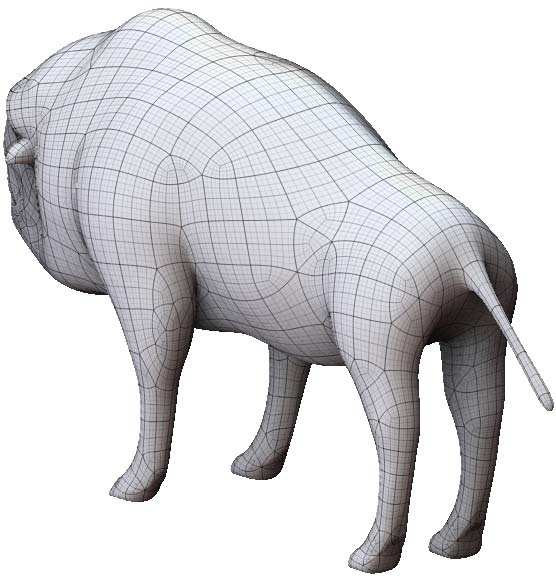
\includegraphics[scale=0.2]{images/basemesh.jpg}
  			\hspace*{0.5cm} 
     		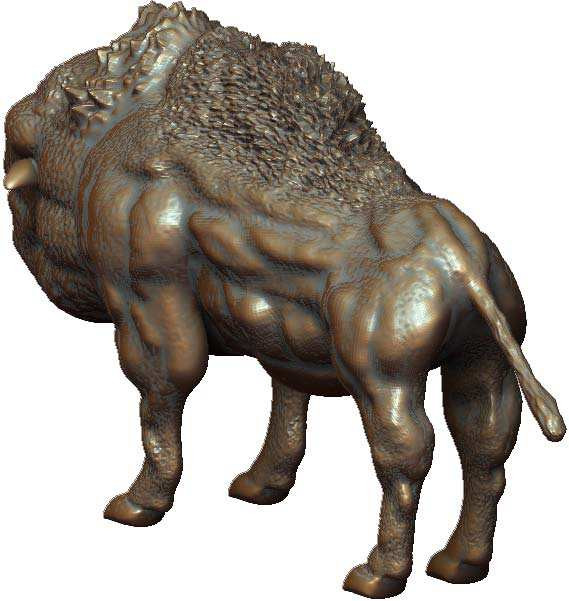
\includegraphics[scale=0.2]{images/detailedmesh.jpg}
     		\hspace*{0.5cm}  
  		}
	\end{figure}
\end{frame}

%% Slide d'introduction
\begin{frame}
	\frametitle{Introduction}
	\begin{block}{Principe du modeleur}
		Générer le maillage d'un objet 3D uniquement à partir de:
		\begin{itemize}
			\item Sphères;
			\item Liens entre ces sphères.
		\end{itemize}
	\end{block}
	
	\begin{block}{Source}
		\begin{center}
			\textit{B-Mesh: A Fast Modeling System for Base Meshes of 3D Articulated Shapes} \\
			Ji Zhongping, Liu Ligang, Wang Yigang \\ 
			
			Institute of Graphics and Image, Hangzhou Dianzi University, China \\
			Department of Mathematics, Zhejiang University, China
		\end{center}
	\end{block}
	
	\begin{center}
		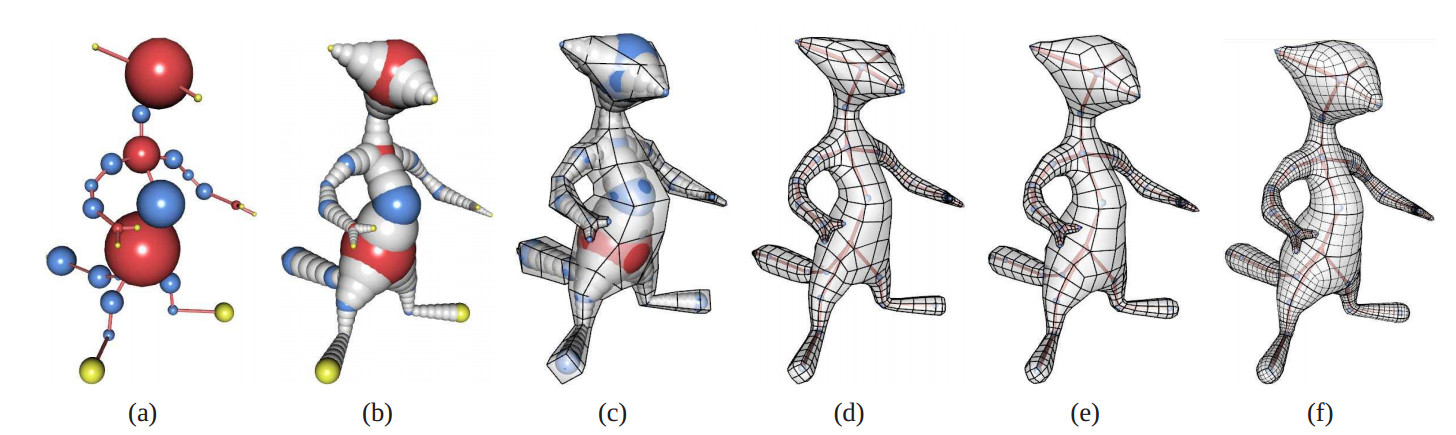
\includegraphics[scale=0.2]{images/bmesh.jpg}
	\end{center}
\end{frame}


%% Interface graphique
\section{Présentation de l'outil}

\begin{frame}
	\frametitle{Sommaire}
	\tableofcontents[currentsection]
\end{frame}

% Slide 1 (screenshot)
\begin{frame}
	\frametitle{Présentation de l'outil}
	\framesubtitle{Aperçu de l'interface graphique}
	\begin{center}
		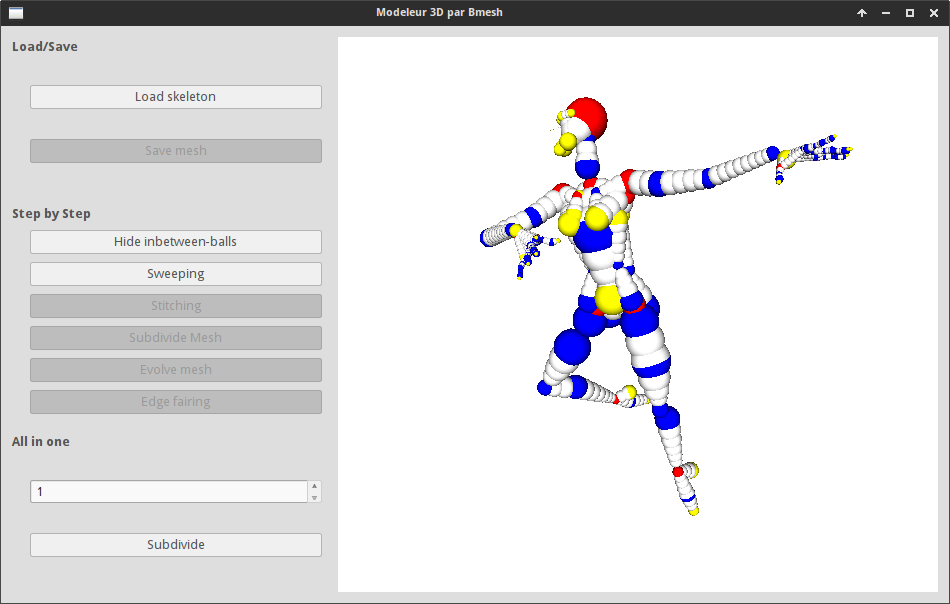
\includegraphics[scale=0.27]{images/screenshot.png}
	\end{center}
\end{frame}

% Slide 2 (description)
\begin{frame}
	\frametitle{Présentation de l'outil}
	\framesubtitle{Fonctionnalités}
	\begin{block}{Chargement / Sauvegarde}
		\begin{itemize}
			\item Chargement d'un squelette (au format .txt)
			\item Sauvegarde du maillage généré (au format .obj)
		\end{itemize}				
	\end{block}
	\begin{block}{Application de l'algorithme}
		\begin{itemize}
			\item Étape par étape...
			\item ... ou tout d'un coup (nombre d'itérations réglable)
		\end{itemize}
	\end{block}
\end{frame}



%% Algorithme
\section{Présentation de l'algorithme}

\begin{frame}
	\frametitle{Sommaire}
	\tableofcontents[currentsection]
\end{frame}


%% Interpolation
\subsection{Interpolation}
\begin{frame}
	\frametitle{Interpolation}
	\begin{block}{But}
		Compléter de manière régulière les segments liant les sphères
	\end{block}
	\begin{block} {Types de sphères}
		\begin{itemize}
			\item \textit{Joint node} (en rouge)
			\item \textit{Connection node} (en bleu)
			\item \textit{End node} (en jaune)
			\item \textit{Inbetween-balls} (en blanc)
		\end{itemize}
	\end{block}
	\begin{center}
	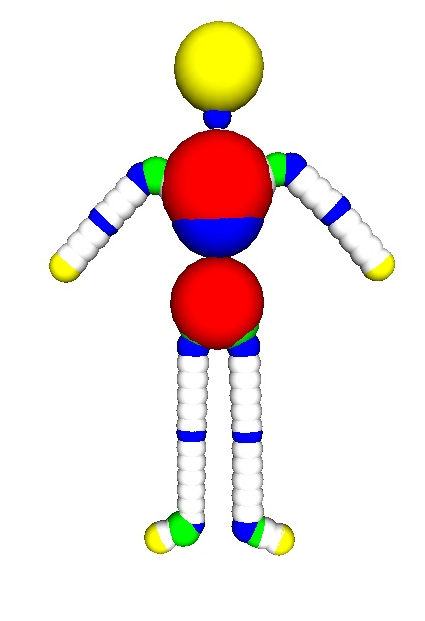
\includegraphics[scale=0.27]{images/bonhomme_interpole.png}
	\end{center}
\end{frame}

%% Sweeping
\subsection{Sweeping}
\begin{frame}
	\frametitle{Sweeping}
	\begin{block}{But}
		Construire un premier maillage autour des branches du squelette
	\end{block}
	\begin{block}{Principe}
		A partir de chaque \textit{joint node}, on parcourt les branches liées à la joint node en entourant les sphères d'un maillage quadrangulaire
	\end{block}
		\begin{figure}[H]
		\centering
		\leavevmode
  		\hbox{
  			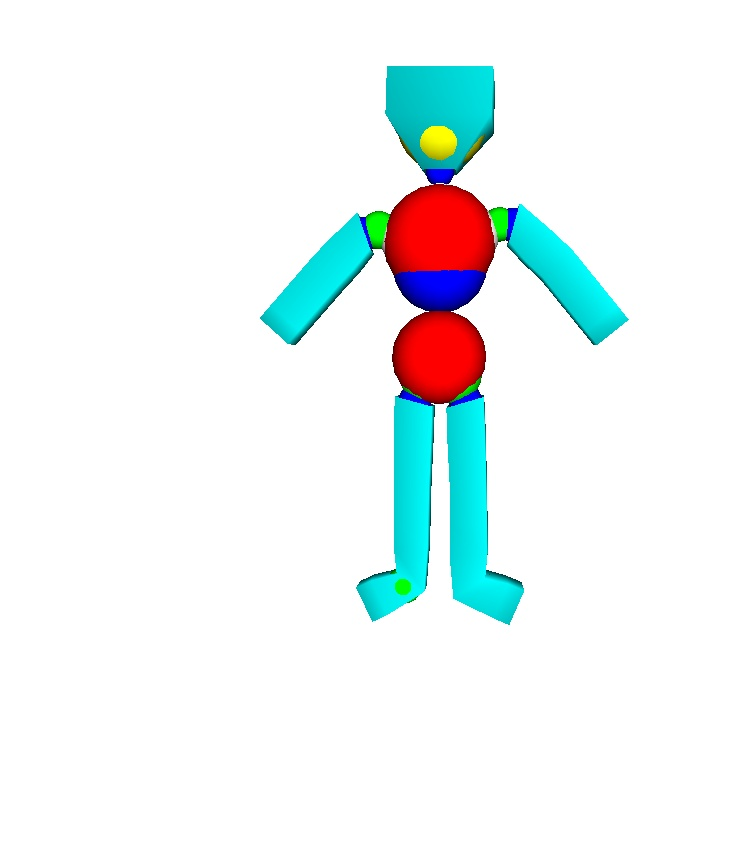
\includegraphics[scale=0.25]{images/sweeping1.jpg}
  			\hspace*{0.5cm} 
     		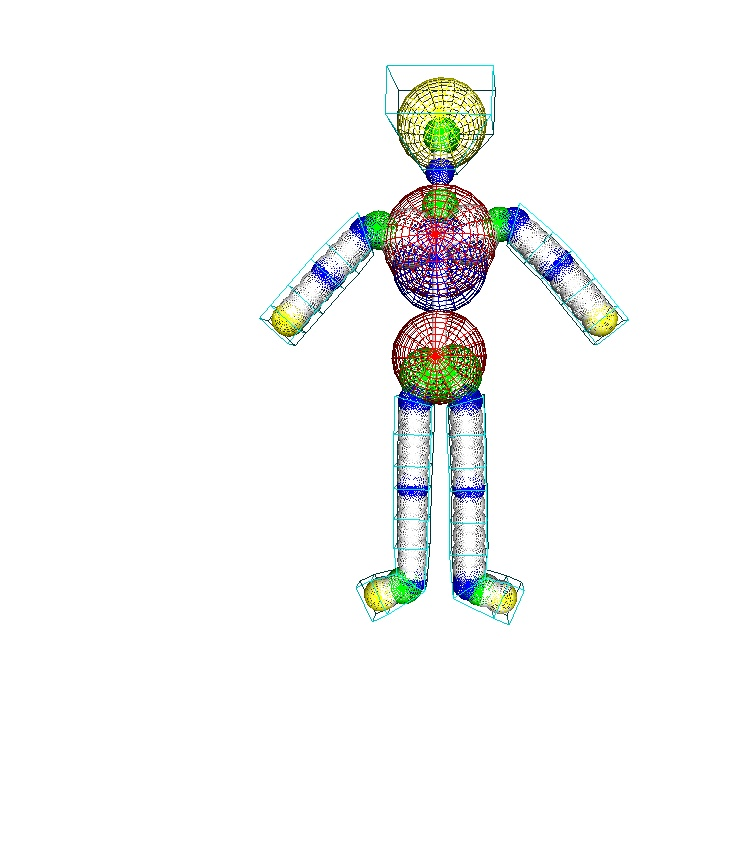
\includegraphics[scale=0.25]{images/sweeping2.jpg}
     		\hspace*{0.5cm}  
  		}
  		\caption{T = 0.1 (à gauche) et T = 0.3 (à droite)}
	\end{figure}
	
\end{frame}

%% Stitching
\subsection{Stitching}
\begin{frame}
	\frametitle{Stitching}
	\begin{block}{But}
		Compléter le premier maillage autour des \textit{joint node}
	\end{block}
	\begin{block}{Principe}
		Pour chaque \textit{joint node} :
		\begin{itemize}
				\item On construit l'enveloppe convexe formée par les points du maillage à l'extrémité des branches liées à la \textit{joint node}
				\item On triangularise l'enveloppe convexe
				\item On passe du maillage triangulaire au maillage quadrangulaire
		\end{itemize}
	\end{block}
	\begin{center}
	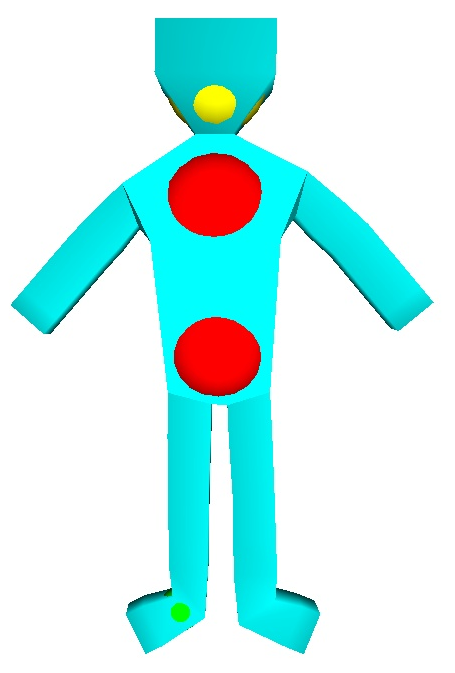
\includegraphics[scale=0.15]{images/stitching.png}
	\end{center}
\end{frame}

%% Tenseur de courbure %%
\begin{frame}
	\frametitle{Tenseur de courbure}
	
	\begin{block}{Définition}
		Courbures et directions principales: valeurs et vecteurs propres de l'endomorphisme symétrique de
		\textbf{Weingarten}
	\end{block}
	
	\begin{block}{Détermination de W}
		\begin{equation*}
			W{(e_i^p)_u \choose (e_i^p)_v} = {(n_i - n_x)_u \choose (n_i - n_x)_v}
		\end{equation*}
		$e_i^p$: projection d'une arête incidente à \textbf{p} dans le plan tangent \\
		$n_i$: normale au point $p_i$ \\
		$((x)_u, (x)_v)$: coordonnées d'un point dans un repère orthonormé du plan tangent
	\end{block}
\end{frame}


%% Subdivision du maillage
\subsection{Subdivision du maillage}
\begin{frame}
	\frametitle{Subdivision du maillage}
	
	\begin{block}{Motivation}
		Avoir un maillage plus fin et plus détaillé
	\end{block}
	
	\begin{block}{Algorithme}
		Algorithme de Catmull-Clark
		\begin{itemize}
			\item algorithme classique;
			\item produit un maillage formé de quadrangles.
		\end{itemize}
	\end{block}
\end{frame}

%% Résultat
\begin{frame}
	\frametitle{Subdivision du maillage}
	\framesubtitle{Résultat}
	
	\begin{center}
		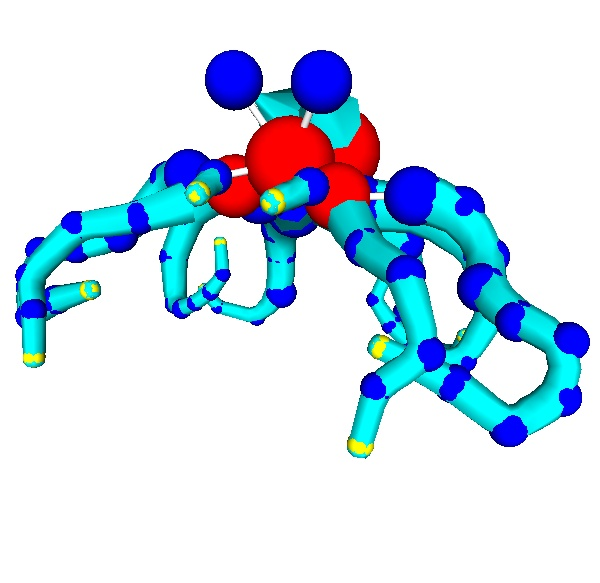
\includegraphics[scale=0.45]{images/catmullclark.jpg}
	\end{center}
\end{frame}


%% Mesh evolution %%
\subsection{Évolution du maillage}

%% Intro
\begin{frame}
	\frametitle{Évolution du maillage}
	\framesubtitle{Quelques notions}
	
	\begin{block}{Motivation}
		Le maillage généré par Catmull-Clark dévie de l'union de sphères.
	\end{block}
	
	\begin{block}{Champ scalaire}
		On définit la fonction $f_i$ par:
		\begin{equation*}
  			f_i(r)=
     			\begin{cases}
        			\left(1 - \left(\frac{r}{R_i}\right)^2 \right)^2 & \text{si $r \le R_i$} \\
        			0 & \text{si $r > R_i$}
     			\end{cases}
		\end{equation*}
		$r^2 = (x - c_x^i)^2 + (y - c_y^i)^2 + (z - c_z^i)^2$ \\
		$R_i = \alpha r_i$, $r_i$ rayon de la sphère $i$ et $\alpha = 1.5$ \\
		$(c_x^i, c_y^i, c_z^i)$ centre de la sphère $i$
	
	\end{block}
\end{frame}

%% évolution suite
\begin{frame}
	\frametitle{Évolution du maillage}
	\framesubtitle{Quelques notions}
	
	\begin{block}{Condition d'arrêt}
		\begin{equation*}
			\mathcal{I}(x) = \sum_{i=1}^{n} f_i - T = 0
		\end{equation*}
	\end{block}
	
	\begin{block}{Équation d'évolution}
		\begin{equation*}
			\frac{d\textbf{x}}{dt} = \textbf{n}(\textbf{x}, t) \mathcal{F}(\textbf{x}, \textbf{n}, \kappa, \mathcal{I}, ...)		
		\end{equation*}
		$\textbf{n} = -\nabla\mathcal{I} / \Vert\nabla\mathcal{I}\Vert$ : normale \\
		$\mathcal{F} = ( \mathcal{I} - \mathcal{I}_{cible} ) f(\kappa)$ : caractérise la vitesse d'évolution \\
		$f(\kappa) = 1 / (1 + |\kappa_1| + |\kappa_2|)$
	\end{block}
\end{frame}

%% évolution fin
\begin{frame}
	\frametitle{Évolution du maillage}
	\framesubtitle{Détermination du nouveau point}
	
	\begin{block}{Nouveau point ?}
		\begin{equation*}
			\textbf{x}(t + dt) = \textbf{x}(t) + \textbf{n}(\textbf{x}, t) \mathcal{F}(\textbf{x}, ...) dt
		\end{equation*}
	\end{block}
	
	\begin{block}{Choix de dt}
		\begin{equation*}
			dt \le \frac{min\{r_i\}}{2^k \mathcal{F}_{max}}
		\end{equation*}
		$k$ : niveau de subdivision
	\end{block}
\end{frame}

%% Résultats
\begin{frame}
	\frametitle{Évolution du maillage}
	\framesubtitle{Résultat}
	
	\begin{figure}[H]
		\centering
		\leavevmode
  		\hbox{
  			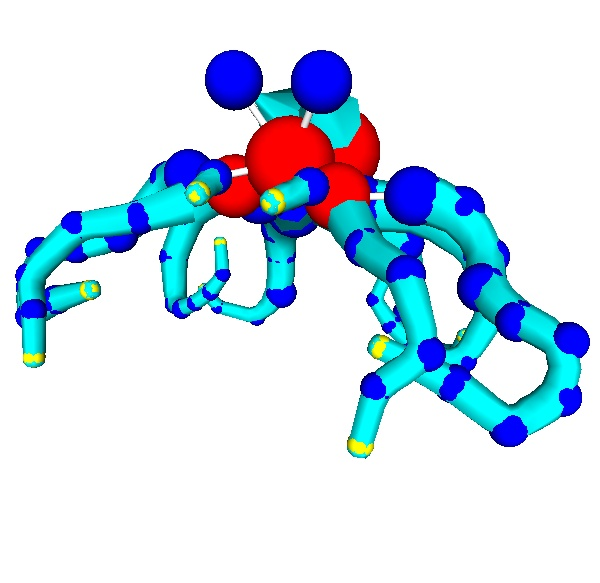
\includegraphics[scale=0.3]{images/catmullclark.jpg}
  			\hspace*{0.5cm} 
     		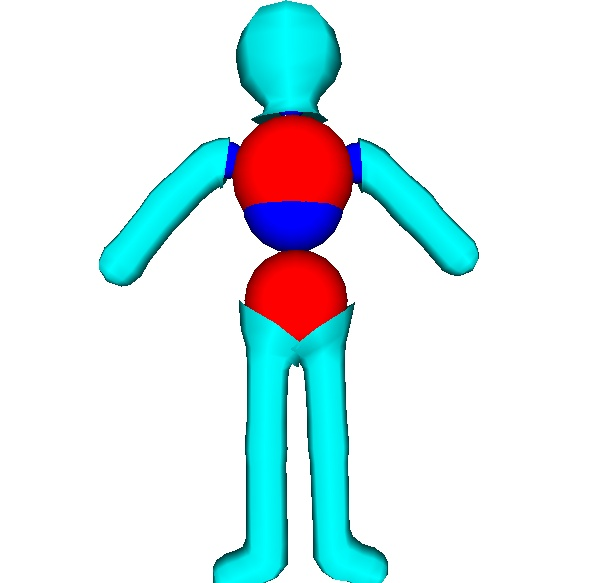
\includegraphics[scale=0.3]{images/meshevolve.jpg}
     		\hspace*{0.5cm}  
  		}
  		\caption{Maillage avant évolution (à gauche) puis après évolution (à droite)}
	\end{figure}
\end{frame}

%% Résultat: influence de T
\begin{frame}
	\frametitle{Résultats}
	\framesubtitle{Influence de T et phénomène de bulge}
	
	\begin{figure}[H]
		\centering
		\leavevmode
  		\hbox{
  			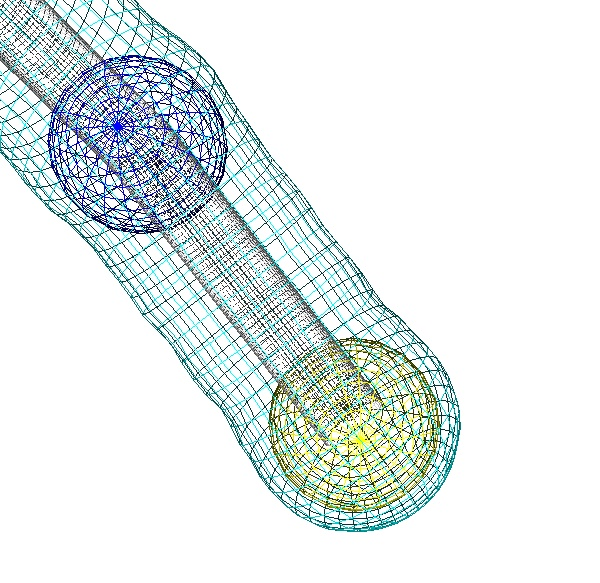
\includegraphics[scale=0.3]{images/evolution_t01.jpg}
  			\hspace*{0.5cm} 
     		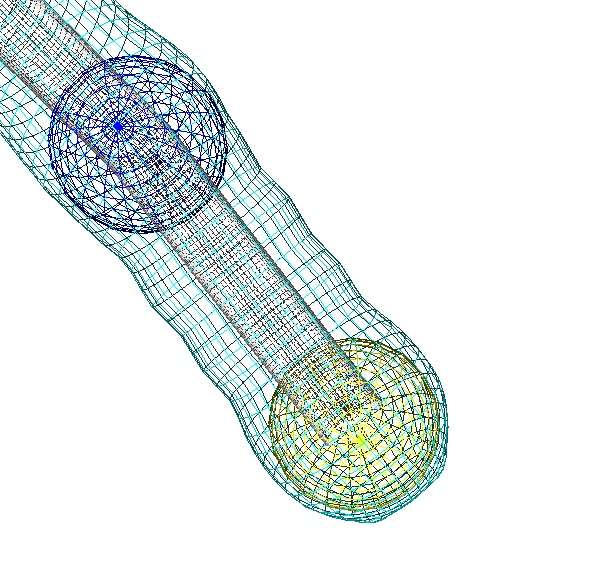
\includegraphics[scale=0.3]{images/evolution_t03.jpg}
     		\hspace*{0.5cm}  
  		}
  		\caption{T = 0.1 (à gauche) et T = 0.3 (à droite)}
	\end{figure}
\end{frame}


%% Edge fairing %%
\subsection{Edge Fairing}

%% Motivation
\begin{frame}
	\frametitle{Edge Fairing}
	\framesubtitle{Motivation}
	
	\begin{block}{Problème de l'évolution}
		Détériore \textit{l'edge flow}
	\end{block}
	
	\begin{block}{Solution ?}
		Appliquer un \textit{fairing} local sur chaque point du maillage.
	\end{block}
	
	\begin{block}{Pré requis}
		Deux types de points:
		\begin{itemize}
			\item les points ayant exactement 4 voisins;
			\item les points n'ayant pas 4 voisins et ceux dont les courbures principales sont identiques.
		\end{itemize}
	\end{block}
\end{frame}

%% Principe
\begin{frame}
	\frametitle{Edge Fairing}
	\framesubtitle{Principe}
	
	\begin{block}{Points de valence 4}
		Pour un point \textbf{p}, minimiser:
		\begin{equation*}
			f(x) = |(a-x).e_v|^2 + |(b-x).e_u|^2 + |(c-x).e_v|^2 + |(d-x).e_u|^2
		\end{equation*}
		avec a,b,c,d projections des voisins de \textbf{p} dans son plan tangent et $e_u, e_v$ directions principales au point 				\textbf{p}
	\end{block}
	
	\begin{block}{Autres points}
		Umbrella operator: approximer le laplacien par $\mathcal{U}(p) = \displaystyle \frac{1}{n} \sum \limits_{i=1}^{n} p_i - p$, avec $p_i$ voisins directs de \textbf{p}.
	\end{block}
\end{frame}


%% Conclusion
\section{Améliorations}
\begin{frame}
	\frametitle{Améliorations}
	
	\begin{block}{Ce qui a été fait}
		\begin{itemize}
			\item Interface graphique;
			\item Sweeping, première étape du stitching, subdivision, évolution et fairing.
		\end{itemize}
	\end{block}
	
	\begin{block}{Ce qui est à améliorer}
		\begin{itemize}
			\item Deuxième étape du stitching;
			\item Meilleures structures de données;
			\item Trouver des solutions aux limitations de l'algorithme.
		\end{itemize}
	\end{block}
\end{frame}


%% références
\section{Références}
\begin{frame}
	\frametitle{Références}
	\begin{itemize}
		\item  Zhongping J., Ligang L., Yigang W., B-mesh: A modeling system for base meshes of 3d articulated shapes, Computer 					Graphics Forum 29 (7) (2010) 2169–2177
		\item Kobbelt L., Campagna S., Vorsatz J., Seidel H.-P.: Interactive multi-resolution modeling on arbitrary meshes. In Proc. of SIGGRAPH (1998), pp. 105–114
	\end{itemize}
\end{frame}






%%%% Fin du document %%%%
\end{document}
